\documentclass[mathserif,usenames,dvipsnames]{beamer}

\usepackage{movie15}
\usepackage{multicol}
\usepackage{beamerthemeshadow}
\usepackage{graphicx}
\usepackage{graphics}
\usepackage{pgf}
\usepackage{tikz, ifthen}
%\usepackage{scalefnt}
\usepgfmodule{shapes}
\usepgfmodule{plot}
\usetikzlibrary{shapes,arrows,shadows,fit}
\usepackage{hyperref}   % Hyperlink references and URLs
\usetikzlibrary{arrows,automata,petri,positioning}
\usepackage[latin1]{inputenc}

%% Hack so 'backup' slides aren't reflected in total slide count
\newcommand{\backupbegin}{
       \newcounter{framenumberappendix}
          \setcounter{framenumberappendix}{\value{framenumber}}
}
\newcommand{\backupend}{
       \addtocounter{framenumberappendix}{-\value{framenumber}}
          \addtocounter{framenumber}{\value{framenumberappendix}} 
}

\title[AHOY: Slide \insertframenumber/\inserttotalframenumber]{AHOY: A Distributed, Event-Based Simulation Environment for Networked Multi-Agent Systems}

\subtitle{Overview}

\author[Ingram \& Rosenfeld]{ 
Dustin~Ingram, Aaron~Rosenfeld, William~Regli}
%% \author[Clark, Ingram, Kolakowska, \& Rosenfeld]{ 
%% Frank~Clark\inst{1}, Dustin~Ingram\inst{1}, Maria~Kolakowska\inst{1}, Aaron~Rosenfeld\inst{1}, William~Regli\inst{1}, Joseph~Macker\inst{2}}

\institute{
%    \inst{1}%
    Drexel University Department of Computer Science, Philadelphia PA\\
%    \inst{2}%
%    US Naval Research Laboratory, Washington DC
}

\date{\today}

\begin{document}

\frame{\titlepage} 

\section{Introduction}
\frame
{
    Problem: Network Simulators \& Agent Simulators are... 
    \begin{itemize}
        \item Separate entities \& applications
        \item Difficult to coordinate
        \item Pre-scripted or pre-computed
        \item Complex to scale
    \end{itemize}
}

\frame
{   
    \frametitle{Abstract}
    \begin{center}
        
\includegraphics[scale=.25]{../common/logo.pdf}
    \end{center}
    \begin{tabular}{l p{8cm}}
        \textit{Abstract:} & AHOY is a distributed, event-based simulation environment designed to test networked multi-agent systems. \\
    \end{tabular}
}

\frame
{
    \frametitle{Extra - Sample Architecture Flow}
    \begin{center}
        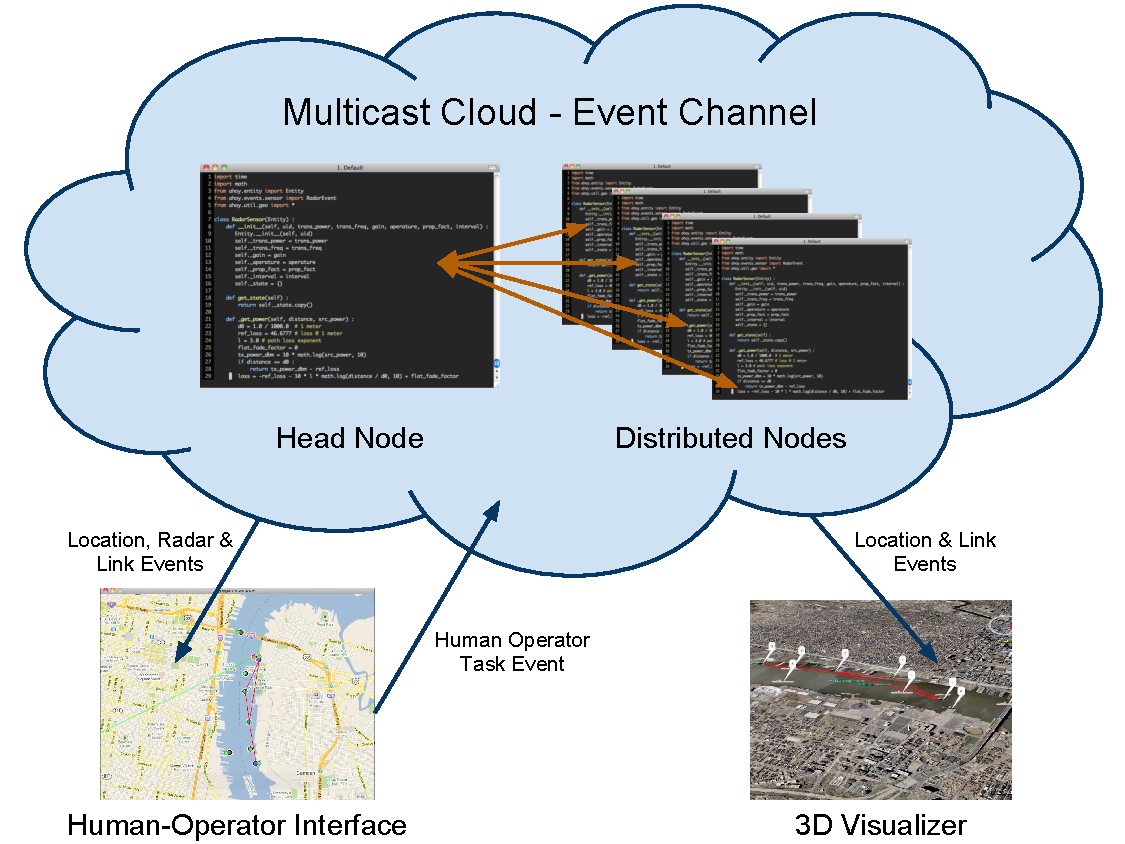
\includegraphics[scale=.48]{../common/demo.pdf}
    \end{center}
}

%\frame
%{
%    \frametitle{Outline}
%    \tableofcontents
%}

\subsection{Background}
%% SVN VISUALIZATION
\section{Development}
\subsection{Features}
\frame
{
    \frametitle{Features}
    \begin{itemize}
        \item Real-time simulation allows for human-in-the-loop interaction
        \item Enable scenarios and network topologies to be easily defined
        \item Make writing custom agents extremely simple
        \item Visualization flexibility
        \item Physically distributed simulation
        \item Entirely event-driven with comprehensive Event API
    \end{itemize}
}

\frame
{
    \frametitle{Event-Based Simulation}
    \begin{itemize}
        \item Every action or change in the simulation is an event
        \item All events are passed over the event channel
        \item Event channel is available to all virtual nodes, agents
        \item Physical nodes as well, including visualizers
        \item New events can be inserted in real-time (human-in-the-loop)
    \end{itemize}
}

%\frame
%{
%    \frametitle{Primary Design Choices}
%    \begin{itemize}
%        \item \textbf{Distribution:}
%        \begin{itemize}
%            \item Physical machines
%            \item Processes
%            \item Threads
%        \end{itemize}
%        \item \textbf{Networking:} 
%        \begin{itemize}
%            \item Common multicast channel
%            \item Pairwise connections (TCP, UDP)
%            \item Delegation Daemons
%        \end{itemize}
%    \end{itemize}
%}
\subsection{Architecture}
\frame
{
    \frametitle{System Architecture Diagram}
    \begin{center}
    \begin{figure}
        \resizebox{0.8\textwidth}{!}{\def\mcwidth{14.5}
\def\mcheight{10}
\tikzstyle{disto} = [minimum height=9cm, minimum width=2.5cm, below of=mc, yshift=-4.2cm, draw, rectangle, rounded corners, fill=gray!30]
\tikzstyle{ntext} = [scale=0.75, yshift=4.65cm, draw, rectangle, rounded corners, fill=white, minimum width=3cm, minimum height=0.55cm]
\tikzstyle{vnode} = [minimum height=1.85cm, minimum width=2cm, text width=1.5cm, draw, rectangle, yshift=-0.25cm, text badly centered, anchor=north, fill=white, densely dotted]
\tikzstyle{agent} = [scale=0.75, yshift=-0.5cm, anchor=north, rectangle, rounded corners, draw, minimum width=2.3cm, minimum height=0.53cm, fill=gray!20]
\tikzstyle{vtext} = [scale=0.75, draw, rectangle, rounded corners, densely dotted, minimum width=3cm, fill=white, anchor=north]
\tikzstyle{start} = [minimum height=1.8cm, minimum width=2cm, text width=1.5cm, draw, rectangle, rounded corners, yshift=2.25cm, text badly centered, fill=gray!10]
\tikzstyle{biggy} = [minimum height=8.4cm, minimum width=2cm, draw, rectangle, rounded corners, yshift=-1.05cm, fill=gray!10]

\begin{tikzpicture}
    \node (mc) [draw, rectangle, rounded corners, dashed] {Multicast Event Channel};
    
    \node (n0) [disto, xshift=-5.5cm] {};
        \node [above of=n0, ntext] {Display Node};
        \node [above of=n0, biggy] {Visualizer};
    
    \node (n1) [disto, xshift=-2.75cm] {};
        \node [above of=n1, ntext] {Head Node};
        \node [above of=n1, biggy] {Simulator};
    
    \node (n2) [disto, xshift=-0cm] {};
        \node [above of=n2, ntext] {Distributed Node};
        \node (sd0) [above of=n2, start] {Startup Daemon};
        \node (vn0) [below of=sd0, vnode, yshift=-0cm] {};
            \node [above of=vn0, vtext] {V. Node 0};
            \node [above of=vn0, agent, yshift=-0.15cm] {Agent 0};
            \node [above of=vn0, agent, yshift=-0.75cm] {Agent 1};
            \node [above of=vn0, agent, yshift=-1.35cm] {Agent 2};
        \node (vn1) [below of=vn0, vnode] {};
            \node [above of=vn1, vtext] {V. Node 1};
            \node [above of=vn1, agent, yshift=-0.15cm] {Agent 0};
            \node [above of=vn1, agent, yshift=-0.75cm] {Agent 1};
            \node [above of=vn1, agent, yshift=-1.35cm] {Agent 2};
        \node (vn2) [below of=vn1, vnode] {};
            \node [above of=vn2, vtext] {V. Node 2};
            \node [above of=vn2, agent, yshift=-0.15cm] {Agent 0};
            \node [above of=vn2, agent, yshift=-0.75cm] {Agent 1};
            \node [above of=vn2, agent, yshift=-1.35cm] {Agent 2};

    \node (n3) [disto, xshift=2.75cm] {};
        \node [above of=n3, ntext] {Distributed  Node};
        \node (sd1) [above of=n3, start] {Startup Daemon};
        \node (vn3) [below of=sd1, vnode, yshift=-0cm] {};
            \node [above of=vn3, vtext] {V. Node 3};
            \node [above of=vn3, agent, yshift=-0.15cm] {Agent 3};
            \node [above of=vn3, agent, yshift=-0.75cm] {Sensor 0};
            \node [above of=vn3, agent, yshift=-1.35cm] {Sensor 1};
        \node (vn4) [below of=vn3, vnode] {};
            \node [above of=vn4, vtext] {V. Node 4};
            \node [above of=vn4, agent, yshift=-0.15cm] {Agent 3};
            \node [above of=vn4, agent, yshift=-0.75cm] {Sensor 0};
            \node [above of=vn4, agent, yshift=-1.35cm] {Sensor 1};
        \node (vn5) [below of=vn4, vnode] {};
            \node [above of=vn5, vtext] {V. Node 5};
            \node [above of=vn5, agent, yshift=-0.15cm] {Agent 3};
            \node [above of=vn5, agent, yshift=-0.75cm] {Sensor 0};
            \node [above of=vn5, agent, yshift=-1.35cm] {Sensor 1};

    \node (n4) [disto, xshift=5.5cm] {};
        \node [above of=n4, ntext] {Distributed  Node};
        \node (sd2) [above of=n4, start] {Startup Daemon};
        \node (vn6) [below of=sd2, vnode, yshift=-0cm] {};
            \node [above of=vn6, vtext] {V. Node 6};
            \node [above of=vn6, agent, yshift=-0.15cm] {Agent 3};
            \node [above of=vn6, agent, yshift=-0.75cm] {Sensor 0};
            \node [above of=vn6, agent, yshift=-1.35cm] {Sensor 1};
        \node (vn7) [below of=vn6, vnode] {};
            \node [above of=vn7, vtext] {V. Node 7};
            \node [above of=vn7, agent, yshift=-0.15cm] {Agent 3};
            \node [above of=vn7, agent, yshift=-0.75cm] {Sensor 0};
            \node [above of=vn7, agent, yshift=-1.35cm] {Sensor 1};
        \node (vn8) [below of=vn7, vnode] {};
            \node [above of=vn8, vtext] {World Object 0};
            \node [above of=vn8, agent, yshift=-0.15cm] {Logic};
    
    \draw[dashed]
        (mc.west) to (-0.5*\mcwidth,0)
        (-0.5*\mcwidth,0) to (-0.5*\mcwidth,-\mcheight)
        (-0.5*\mcwidth,-\mcheight) to (0.5*\mcwidth,-\mcheight)
        (0.5*\mcwidth,-\mcheight) to (0.5*\mcwidth,0)
        (0.5*\mcwidth,0) to (mc.east);

\end{tikzpicture}
}
    \end{figure}
    \end{center}
}


%\section{Demo: Delaware River Scenario}
\subsection{Scenarios}
%\frame
%{
%    \frametitle{Outline}
%    \tableofcontents
%}

\frame
{
    \frametitle{Scenarios}
    Possible scenarios:
    \begin{itemize}
        \item Communication \& coordination of first responders
        \item Unmanned cars in highway traffic
        \item Load evaluation of large WiFi network
    \end{itemize}
    Our scenario:
    \begin{itemize}
        \item Threat detection and crisis avoidance on Delaware River
    \end{itemize} 
}

\frame
{
    \frametitle{Delaware River Scenario}
    \begin{itemize}
        \item AIS data for large commercial ships
        \item ``Markov Model'' agent
        \item ``Threat Ship'' agent
        \item Radar \& Sonar sensor models
        \item ``Threat Detection'' agent
        \item ``UAV'' agent
        \item Camera sensor model
        \item Chemical sensor model

    \end{itemize}
}

\frame
{
    \frametitle{Videos}
    \begin{itemize}
        \item \href{http://cs.drexel.edu/~dsi23/act1.ogv}{Act I: Threat Detection, Sensor Correlation}
        \item \href{http://cs.drexel.edu/~dsi23/act2.ogv}{Act II: Human-Agent Interaction, Threat Validation}
        \item \href{http://cs.drexel.edu/~dsi23/act3.ogv}{Act III: Sensor Evaluation, Behavior Modification}
    \end{itemize}
}

\section{Future Work}
\frame
{
    \frametitle{Future Work}
    Networking \& Network Models
    \begin{itemize}
        \item ``Routing/Router'' agent, etc.
    \end{itemize}
    Library of realistic Sensor \& Agent models
    \begin{itemize}
        \item Reusable for multiple scenarios 
    \end{itemize}
    Physical Models:
    \begin{itemize}
        \item Terrain: Land \& Water effects 
        \item 3D Models: Nodes, ships, buildings, etc.
    \end{itemize}
}

%% AIS Data images
%\frame
%{
%    \begin{center}
%        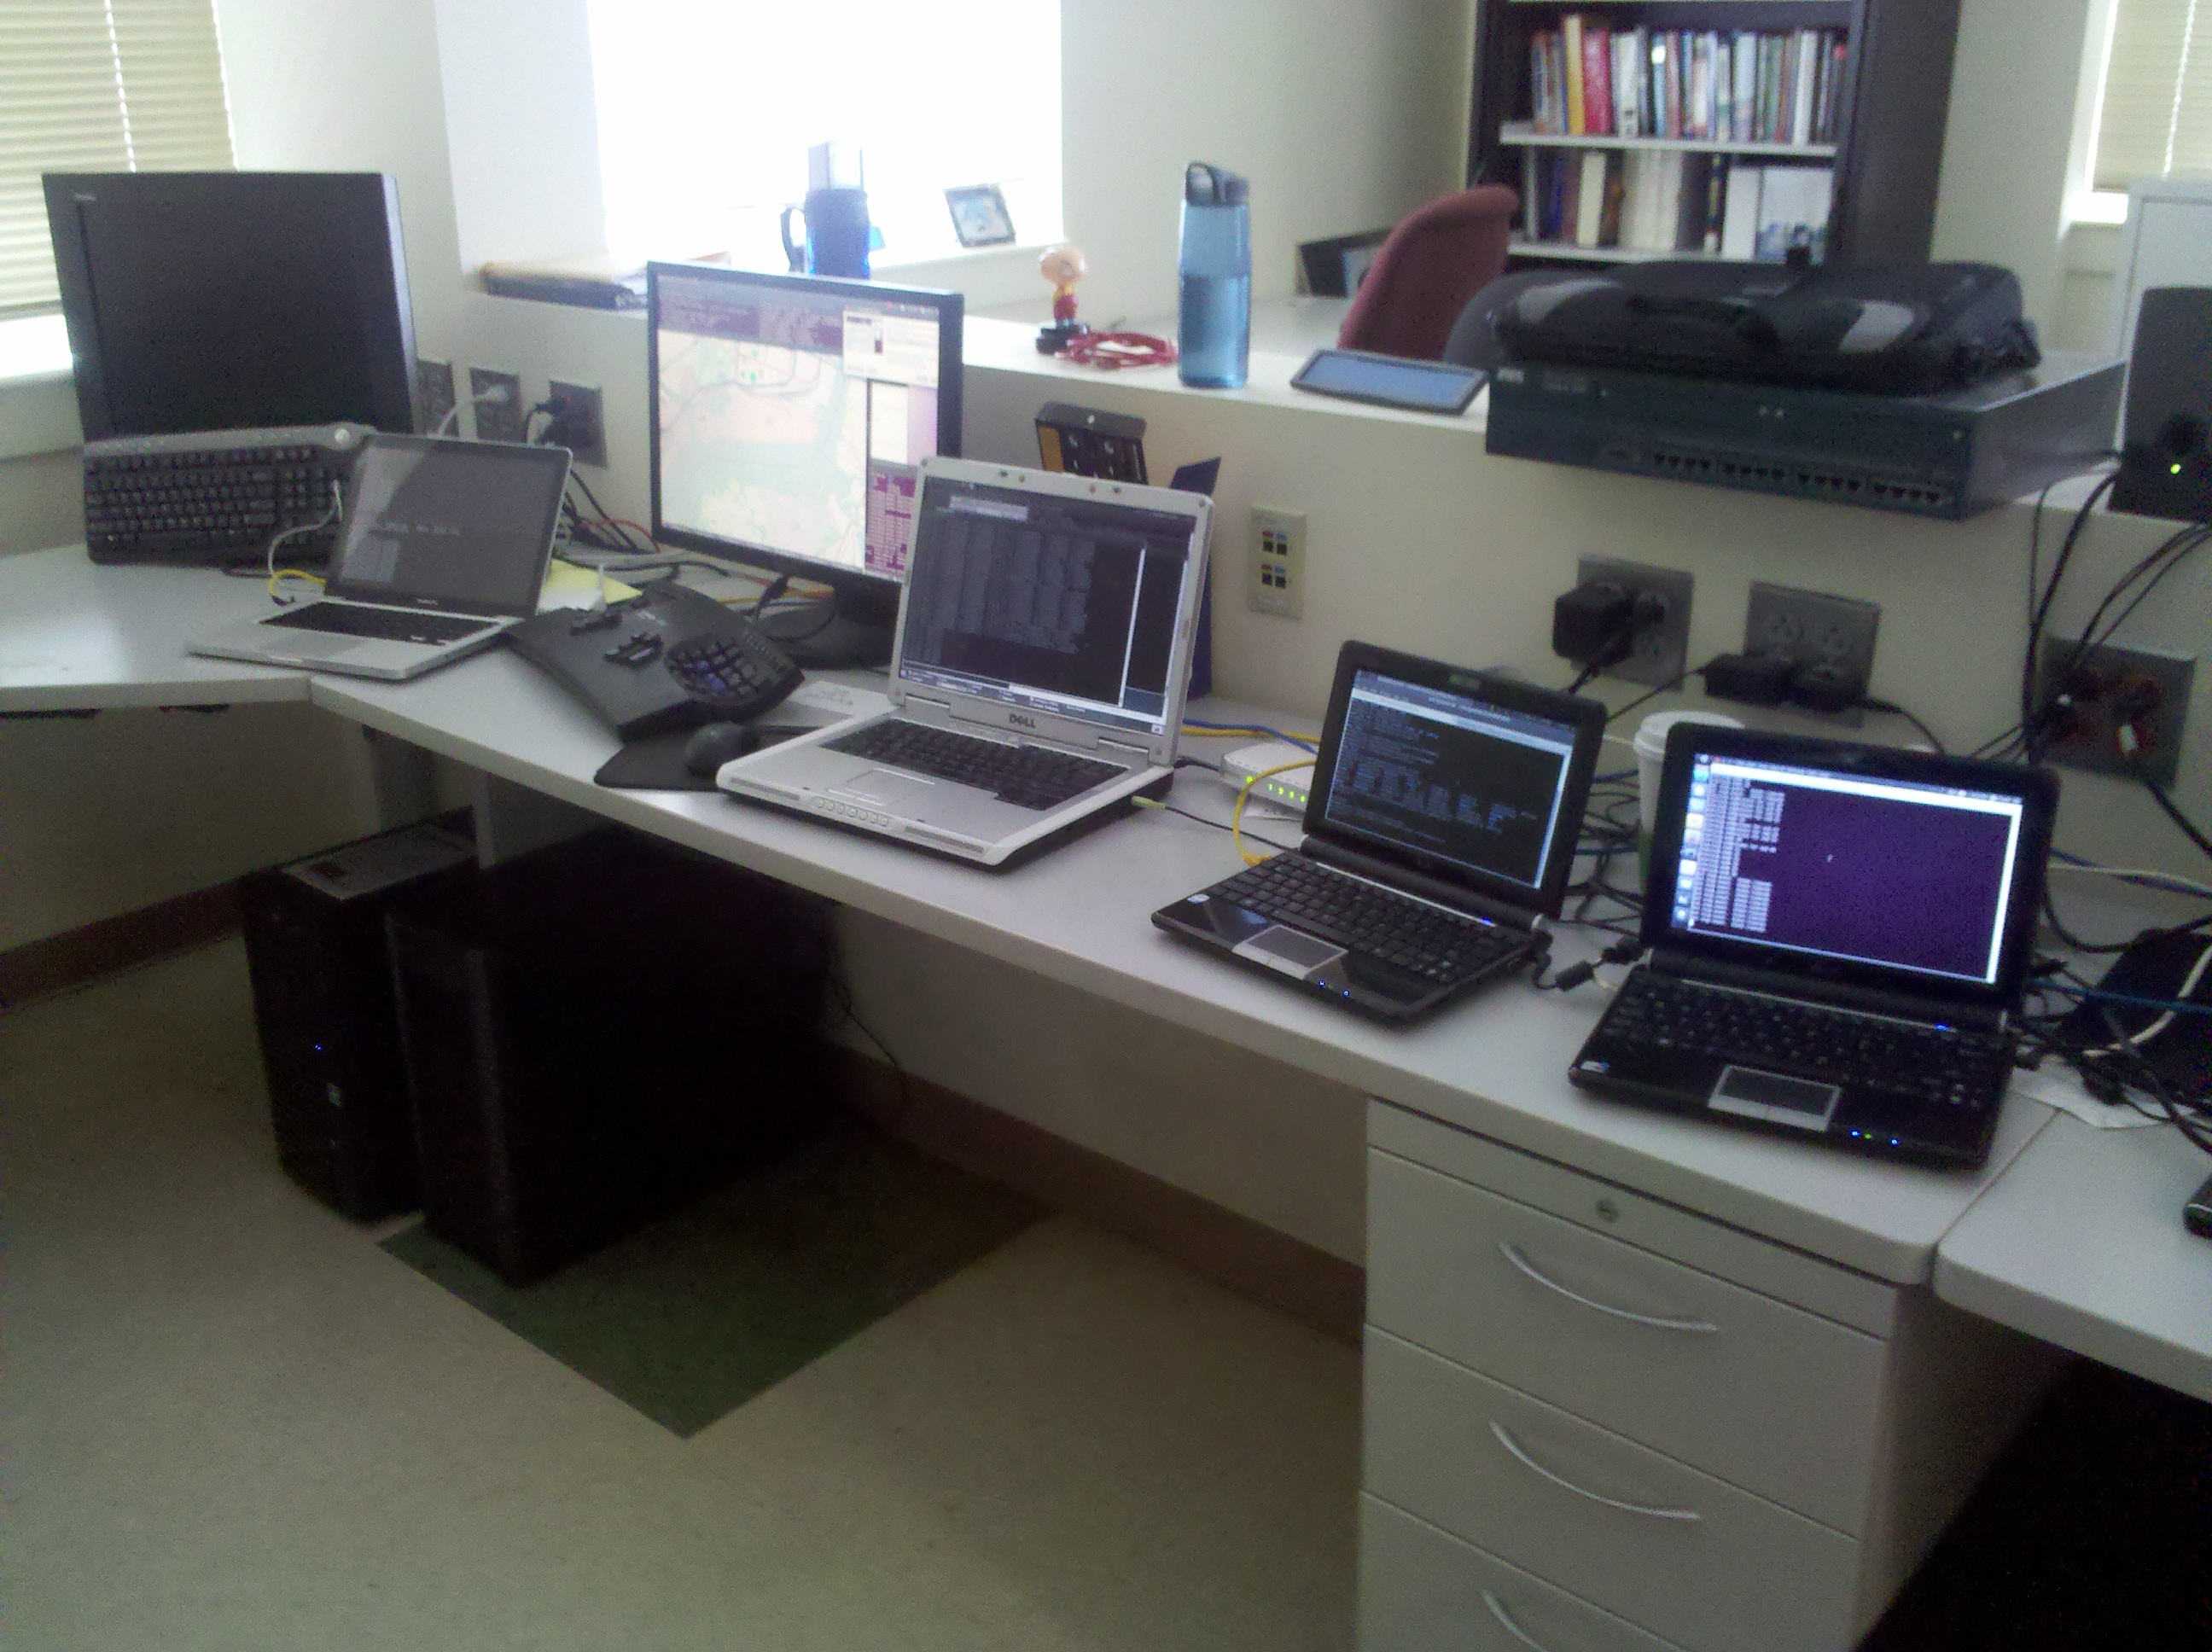
\includegraphics[scale=.1]{../common/testbed.jpg}
%    \end{center}
%}
%\subsection{Act I}
%\frame
%{
%    \frametitle{Act I: Threat Detection, Sensor Correlation}
%    Agent uses Radar and Sonar sensors to detect threats to AIS ships:\\
%    \begin{itemize}
%        \item AIS ships are moving based on Markov models
%        \item Small boats are moving up/down river
%        \item Sonar \& Radar sensors on riverbanks
%        \item Threat agent uses sensors to detect non-AIS boats 
%        \item Agent alerts human operator to potential threats
%    \end{itemize}
%}
%% Act 1 Video
%\subsection{Act II}
%\frame
%{
%    \frametitle{Act II: Human-Agent Interaction, Threat Validation}
%    Human operator commands autonomous UAV agent to improve data accuracy with Camera sensor:
%    \begin{itemize}
%        \item Threat has been detected by threat agent 
%        \item Human operator initiates UAV flyover of specific region
%        \item UAV uses camera to provide more accurate position of threat
%    \end{itemize}
%}
%%% Act 2 Video
%\subsection{Act III}
%\frame
%{
%    \frametitle{Act III: Sensor Evaluation, Behavior Modification}
%    Chemical sensors detect oil spill while human operator diverts AIS ships:
%    \begin{itemize}
%        \item AIS tanker is destroyed by threat causing chemical spill
%        \item Spill activates chemical sensors \& restricts shipping channel
%        \item Human operator plans alternative route based on sensor data
%        \item Alternative route is sent to AIS ships via radio link
%    \end{itemize}
%}
%% Act 3 Video
%\section{Demo: Predator/Prey}
%\frame
%{
%    \frametitle{Outline}
%    \tableofcontents
%}
%
%\frame
%{
%    \frametitle{CS485/511 Robot Lab: Predator/Prey Assignment}
%    \begin{itemize}
%        \item Autonomous multi-agent team coordination
%        \item Random environment, limited sensor
%        \item Predators' shared goal: Efficient capture of Prey
%    \end{itemize}
%}
%
%\frame
%{
%    \frametitle{CS485/511 Robot Lab: Predator/Prey Assignment}
%    \begin{center}
%    \begin{tabular}{|c|c|} \hline
%        \textbf{Agent Implementation} & \textbf{Avg. Time to Catch Prey} \\ \hline
%        Predator 1 & 202 seconds\\ \hline
%        Predator 2 & 145 seconds\\ \hline
%        Predator 3 & 132 seconds\\ \hline
%    \end{tabular}
%    \end{center}
%}
%
%\section{Conclusion}
%\frame
%{
%    \frametitle{Impact}
%    \begin{itemize}
%        \item Research Tool
%        \item Educational Tool
%        \item Cost
%        \item Time
%    \end{itemize}
%}
%
%
%\frame
%{
%    \frametitle{Challenges}
%    \begin{itemize}
%        \item Demonstration required completing an additional project:
%        \begin{itemize}
%            \item Creating realistic sensor models (Radar, Sonar, Camera)
%            \item Designing GUI \& human interface from scratch
%            \item Creating intelligent \& functioning agents
%        \end{itemize}
%        \item Testing:
%        \begin{itemize}
%            \item Difficult to test without accompanying scenario
%            \item Scenario may introduce additional bugs
%            \item Code coverage is complicated across distributed systems
%        \end{itemize}
%    \end{itemize}
%}
%
%\frame
%{
%    \frametitle{Originality}
%    \begin{quote}
%        \small 
%        ``There is a number of platforms that facilitate the development of agent based systems [...] Looking from another perspective, the research area of network simulators is a well established one. Although these simulators provide high fidelity simulation of network properties, they are by no means agent-oriented. An integration with one of the agent enabling platforms seems to be a non trivial problem. However, there is a recently started project AHOY that aims to employ network simulators of this kind in multi-agent simulation.''
%    \end{quote}
%    \vspace{0.5cm}
%    \tiny
%    -- Michal \v{C}\'{a}p, Ji\v{r}\'{i} Vok\v{r}\'{i}nek, Anton\'{i}n Komenda: Communication- and Computation- Bounded Agents in Multi-Agent Simulations. In: Proceedings of HoloMAS, the International Conference on Industrial Applications of Holonic and Multi-Agent Systems, 2011.
%
%}

\frame
{
    \frametitle{Contact \& Links}
    \begin{tabular}{l l}
        \textbf{Website:} & http://ahoy.googlecode.com/ \\
        & \\
        \textbf{Team:} & Dustin S. Ingram - \texttt{dustin@cs.drexel.edu} \\
        & Aaron M. Rosenfeld - \texttt{ar374@cs.drexel.edu} \\
        & \\
        \textbf{Advisor:} & William C. Regli - \texttt{regli@cs.drexel.edu} \\
    \end{tabular}
    \vspace{0.75cm}
    \begin{center}
    \begin{tabular}{c c c c}
    
\includegraphics[scale=.28]{../common/drexel.pdf} & 
\includegraphics[scale=.33]{../common/nrl.png} & 
\includegraphics[scale=.125]{../common/acin.pdf} & 
\includegraphics[scale=.125]{../common/cvut.png} \\
    \end{tabular}
    \end{center}

}

%% Begin backup slides
\backupbegin

\frame
{
    \begin{center}
        \includegraphics[scale=.5]{../mindmap/mindmap1.pdf}
    \end{center}
}

\frame
{
    \begin{center}
        \includegraphics[scale=.75]{../mindmap/mindmap2.pdf}
    \end{center}
}

\frame
{
    \begin{center}
        \includegraphics[scale=.55]{../mindmap/mindmap3.pdf}
    \end{center}
}

\frame
{
    \frametitle{Extra - Background on Network Simulators}
    \begin{itemize}
        \item Application and protocol testing without physical hardware
        \item Mimic the properties of a physical network
        \item Network compents are virtualized (``nodes'') 
        \item Allow multiple virtual nodes to run on one physical machine
        \item Scale well, easy to re-configure
        \item Cost \& time effective
    \end{itemize}
}

\frame
{
    \frametitle{Extra - Background on Agents \& Agent Frameworks}
    \begin{block}{Definition}
    An \emph{intelligent agent} is software which observes and acts upon an environment and directs its activity towards achieving goals (Russell, Norvig).
    \end{block}

    \textbf{Agent Simulators}
    \begin{itemize}
        \item Used to test agent algorithms within virtual worlds
        \item Rules define actions to be taken based on beliefs
        \item Agent rule-sets react to sensory information in the world
        \item Allows for large-scale simulation unfeasible in the real-world
    \end{itemize}
}


\frame
{
    \frametitle{Extra - Alternatives}
    \footnotesize
    \textbf{Networks}
    \begin{itemize}
        \item NS2 (http://www.isi.edu/nsnam/ns)
        \item NS3 (http://www.nsnam.org)
        \item CORE (http://cs.itd.nrl.navy.mil/work/core)
        \item MANE (http://cs.itd.nrl.navy.mil/work/mane)
        \item EMANE (http://cs.itd.nrl.navy.mil/work/emane)
        \item QualNet (http://www.scalable-networks.com/products/qualnet)
    \end{itemize}

    \textbf{Agents}
    \begin{itemize}
        \item AGLOBE (http://agents.felk.cvut.cz/aglobe)
        \item AgentFly (http://agents.felk.cvut.cz/projects)
        \item Player/Stage (http://playerstage.sourceforge.net)
        \item JADE (http://jade.tilab.com)
        \item NetLogo (http://ccl.northwestern.edu/netlogo)
        \item MASON (http://www.cs.gmu.edu/~eclab/projects/mason)
    \end{itemize}
}

\frame
{
    \frametitle{Extra - Radar Specifics}
    \small
    Given a transmit power $P_t$, antenna gain $G_t$, aperture area $A_r$, target cross-sectional area $\sigma$, propagation factor $F$, and time to receive reflected wave $t$.      Distance to closest non-occluded entity in each sweep:
    {\footnotesize
    \begin{align*}
        d = \frac{t \cdot c}{2}
    \end{align*}
    }
    Entity's location $\left(\phi_t, \lambda_t\right)$ can be estimated with:
    {\footnotesize
    \begin{align*}
        \phi_t = sin^{-1}\left(sin\left(\phi_r\right) \cdot cos\left(d/R_{e}\right) + cos\left(\phi_r\right) \cdot sin\left(d/R_{e}\right) \cdot cos\left(\theta\right)\right) \\ 
        \lambda_t = \lambda_t + tan^{-1}\left(sin\left(\theta\right) \cdot sin\left(d/R_{e}\right) \cdot cos\left(\phi_r\right), cos\left(d/R_{e}\right)-sin\left(\phi_r\right) \cdot sin\left(\phi_t\right)\right)
    \end{align*}
    }
    An estimate of velocity is calculated by the Doppler equation:
    {\footnotesize
    \begin{align*}
        \left|\vec{v_{\parallel}}\right| = -\frac{c \cdot \left(f_{recv} - f_{trans}\right)}{f_{trans}}.
    \end{align*}
    }
    Further, pathloss of radio waves is incorporated. If $P_r$ falls below the sensitivity of the antenna, the target will not be detected.
    {\footnotesize
    \begin{align*}
        P_r = \frac{P_t G_t A_r \sigma F^4}{\left(4 \pi\right)^4 d^4}
    \end{align*}
    }
}

\frame
{
    \frametitle{Extra - Sonar Specifics}
    \small
    Given a sonar source transformed into cartesian coordinates $(x_s, y_s, z_s)$ and entity at $(x_e, y_e, z_e)$, the round-trip time of sound is given by:
    \begin{align*}
        \Delta t = \int\limits_{z_s}^{z_e}{s(z) \cdot \sqrt{1 + \left(\frac{\Delta x}{\Delta z}\right)^2} \mathrm{d}z}
    \end{align*}
    Signal-to-noise ratio is given by:
    \begin{align*}
        \frac{S}{N} = L_s - 20 \cdot log(d) + L_t - \mathcal{N}(n_\mu, n_\sigma) - 10 \cdot log(S_b)
    \end{align*}
    Where $L_s$ is the source level, $d$ is the distance between the sonar and an entity, $L_t$ is the target level, $\mathcal{N}$ is a normal distribution, and $S_b$ is the source bandwidth.  If the SNR falls below a certain threshold, sonar will not pick up an entity.
}

\frame
{
    \frametitle{Extra - Log Loss Links}
    In the log-loss model of radio propagation, the received signal strength is given by:
    \begin{align*}
        P_{rx} = P_{tx} - l_0 - 10 \cdot \gamma log(\frac{d}{d_0}) + \chi
    \end{align*}
    Where $P_{tx}$ is the transmission power, $\gamma$ is a path loss exponent, $l_0$ the loss at a reference distance $d_0$, and $\chi$ is a flat-fading factor.

    If $P_{rx}$ falls below a threshold, the interface will not receive the data.
}

%% End backup slides
\backupend

\end{document}
